\documentclass[border=15pt, multi, tikz]{standalone}

\usepackage{tikz}
\usetikzlibrary{quotes,arrows.meta}
\usetikzlibrary{positioning}
\def\edgecolor{rgb:blue,4;red,1;green,4;black,3}
\newcommand{\midarrow}{\tikz \draw[-Stealth,line width =0.8mm,draw=\edgecolor] (-0.3,0) -- ++(0.3,0);}
\usepackage{Box}
\usepackage{RightBandedBox}

\def\ConvColor{rgb:blue,5;green,2.5;white,5}
\def\ConvReluColor{rgb:blue,5;green,5;white,5}
\def\PoolColor{rgb:red,1;black,0.3}
\def\DcnvColor{rgb:blue,5;green,2.5;white,5}
\def\UnpoolColor{rgb:yellow,5;red,2.5;white,5}
\def\SoftmaxColor{rgb:magenta,5;black,7}
\usepackage{xcolor}
\usetikzlibrary{3d} %for including external image 

\begin{document}

\begin{tikzpicture}
\tikzstyle{connection}=[ultra thick,every node/.style={sloped,allow upside down},draw=\edgecolor,opacity=0.7]
%%%%%%%%%%%%%%%%%%%%%%%%%%%%%%%%%%%%%%%%%%%%%%%%%%%%%%%%%%%%%%%%%%%%%%%%%%%%%%%%%%%%%%%%
%% Draw Layer Blocks
%%%%%%%%%%%%%%%%%%%%%%%%%%%%%%%%%%%%%%%%%%%%%%%%%%%%%%%%%%%%%%%%%%%%%%%%%%%%%%%%%%%%%%%%
%%%%%%%%%%   
\node (image) at (0,0,0) {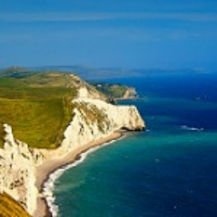
\includegraphics[width=4cm,height=4cm]{img/sub-img/landscape-example.png}};

\node (tab) at (5,0,0) {
    \begin{tabular}{|c|}
        \hline
        Forest \\
        \hline
        {\color{red}\textbf{Sea}} \\
        \hline
        Street \\
        \hline
        Mountain \\
        \hline
        Glacier \\
        \hline
        Building \\
        \hline
        
    \end{tabular}
};

%Connections

\path[->,>=stealth,line width=5pt] (image) edge node [left] {} (tab);

\end{tikzpicture}
\end{document}\grid
